\documentclass[14pt]{beamer}
\usepackage{./Estilos/BeamerUVM}
\usepackage{./Estilos/ColoresLatex}
%Sección para el tema de beamer, con el theme, usercolortheme y sección de footers
\usetheme{Berlin}
\usecolortheme{beaver}
%\useoutertheme{default}
\setbeamercovered{invisible}
% or whatever (possibly just delete it)
\setbeamertemplate{section in toc}[sections numbered]
\setbeamertemplate{subsection in toc}[subsections numbered]
\setbeamertemplate{subsection in toc}{\leavevmode\leftskip=3.2em\rlap{\hskip-2em\inserttocsectionnumber.\inserttocsubsectionnumber}\inserttocsubsection\par}
% \setbeamercolor{section in toc}{fg=blue}
% \setbeamercolor{subsection in toc}{fg=blue}
% \setbeamercolor{frametitle}{fg=blue}
% \setbeamertemplate{caption}[numbered]

\setbeamertemplate{footline}
\beamertemplatenavigationsymbolsempty
\setbeamertemplate{headline}{}


\makeatletter
% \setbeamercolor{section in foot}{bg=gray!30, fg=black!90!orange}
% \setbeamercolor{subsection in foot}{bg=blue!30!yellow, fg=red}
% \setbeamercolor{date in foot}{bg=black, fg=white}
\setbeamertemplate{footline}
{
  \leavevmode%
  \hbox{%
  \begin{beamercolorbox}[wd=.333333\paperwidth,ht=2.25ex,dp=1ex,center]{section in foot}%
    \usebeamerfont{section in foot} \insertsection
  \end{beamercolorbox}%
  \begin{beamercolorbox}[wd=.333333\paperwidth,ht=2.25ex,dp=1ex,center]{subsection in foot}%
    \usebeamerfont{subsection in foot}  \insertsubsection
  \end{beamercolorbox}%
  \begin{beamercolorbox}[wd=.333333\paperwidth,ht=2.25ex,dp=1ex,right]{date in head/foot}%
    \usebeamerfont{date in head/foot} \insertshortdate{} \hspace*{2em}
    \insertframenumber{} / \inserttotalframenumber \hspace*{2ex} 
  \end{beamercolorbox}}%
  \vskip0pt%
}

% \usefonttheme{serif}
\usepackage[clock]{ifsym}
\usepackage{pstricks-add}
\DeclareSIUnit\erg{erg}
\DeclareSIUnit[number-unit-product = {\,}]\cal{cal}

\sisetup{per-mode=symbol}
\resetcounteronoverlays{saveenumi}

% Macro para agregar el logo de UVM en cada slide de la presentación

\addtobeamertemplate{frametitle}{}{%
\begin{tikzpicture}[remember picture,overlay]
\coordinate (logo) at ([xshift=-1.5cm,yshift=-0.8cm]current page.north east);
% \fill[devryblue] (logo) circle (.9cm);
% \clip (logo) circle (.75cm);
\node at (logo) {
\includegraphics[width=2.1cm]{Imagenes/logo_UVM.png}};
\end{tikzpicture}}


\title{\Large{Física y Contaminación} \\ \normalsize{Física III}}
\date{}

\begin{document}
\maketitle

\section*{Contenido}
\frame[allowframebreaks]{\frametitle{Contenido} \tableofcontents[currentsection, hideallsubsections]}

\section{Evento importante}
\frame{\tableofcontents[currentsection, hideothersubsections]}
\subsection{Involucramiento}

\begin{frame}
\frametitle{El 22 de abril}
Este día se celebra el \textocolor{dartmouthgreen}{Día Internacional de la Madre Tierra}.
\end{frame}
\begin{frame}
\frametitle{¿Por qué es importante?}
Cada año, en este día se busca crear una conciencia común a los problemas de:
\pause
\setbeamercolor{item projected}{bg=ecru,fg=black}
\setbeamertemplate{enumerate items}{%
\usebeamercolor[bg]{item projected}%
\raisebox{1.5pt}{\colorbox{bg}{\color{fg}\footnotesize\insertenumlabel}}%
}
\begin{enumerate}[<+->]
\item Sobrepoblación.
\item Contaminación.
\seti
\end{enumerate}
\end{frame}
\begin{frame}
\frametitle{¿Por qué es importante?}
\setbeamercolor{item projected}{bg=ecru,fg=black}
\setbeamertemplate{enumerate items}{%
\usebeamercolor[bg]{item projected}%
\raisebox{1.5pt}{\colorbox{bg}{\color{fg}\footnotesize\insertenumlabel}}%
}
\begin{enumerate}[<+->]
\conti
\item Conservación de la biodiversidad.
\item Calentamiento global.
\item Otras preocupaciones ambientales para proteger la Tierra.
\end{enumerate}
\end{frame}
\begin{frame}
\begin{figure}
    \centering
    
\includegraphics[scale=0.2]{Imagenes/dia_internacional_madre_tierra.jpg}
\end{figure}
\end{frame}

\section{Actividad a realizar}
\frame{\tableofcontents[currentsection, hideothersubsections]}
\subsection{Elaboración de un poster}

\begin{frame}
\frametitle{Actividad a desarrollar}
Como parte de la celebración del \textocolor{dartmouthgreen}{Día Internacional de la Madre Tierra}, \pause tendrás que elaborar un poster con el tema de \textocolor{electricindigo}{contaminación} y de \textocolor{ferrarired}{medidas para reducir o eliminar la misma}.
\end{frame}

\subsection{Temas a presentar}

\begin{frame}
\frametitle{Temas para el poster}
Se desarrollará un tema en el poster a partir de los siguientes:
\end{frame}
\begin{frame}
\frametitle{Contaminación por Pilas/Baterías}
\vspace*{-1cm}
\begin{figure}
    \centering
    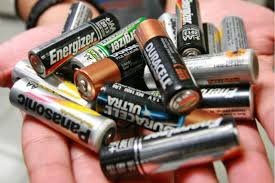
\includegraphics[scale=0.75]{Imagenes/Contaminacion_01.jpg}
\end{figure}
\end{frame}
\begin{frame}
\frametitle{Contaminación del Agua}
\vspace*{-1cm}
\begin{figure}
    \centering
    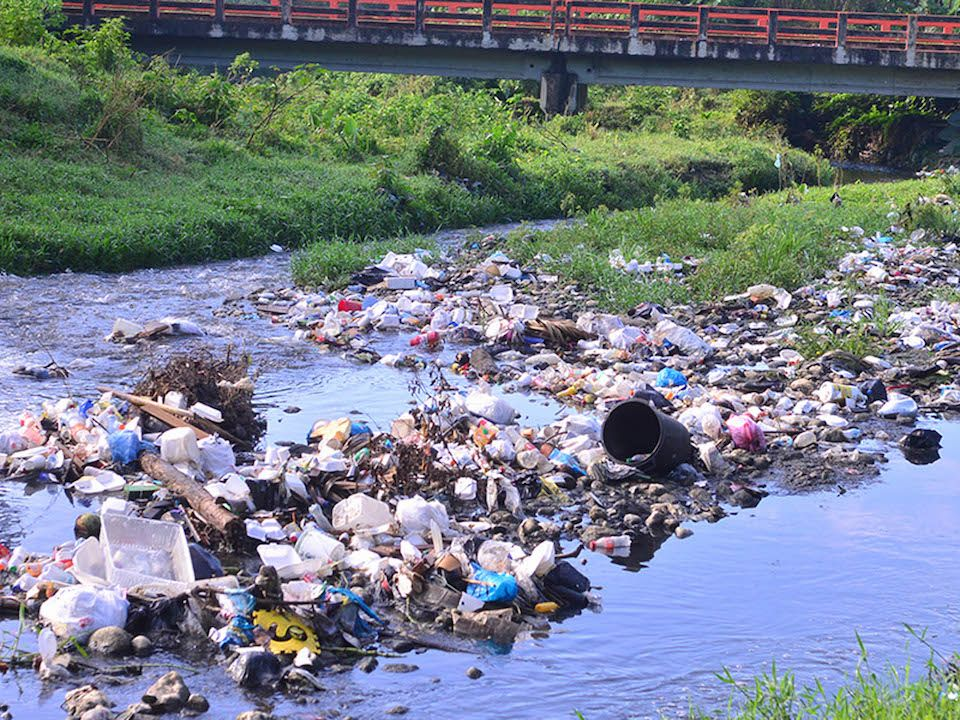
\includegraphics[scale=0.35]{Imagenes/Contaminacion_02.jpg}
\end{figure}
\end{frame}
\begin{frame}
\frametitle{Contaminación del Suelo}
\vspace*{-1cm}
\begin{figure}
    \centering
    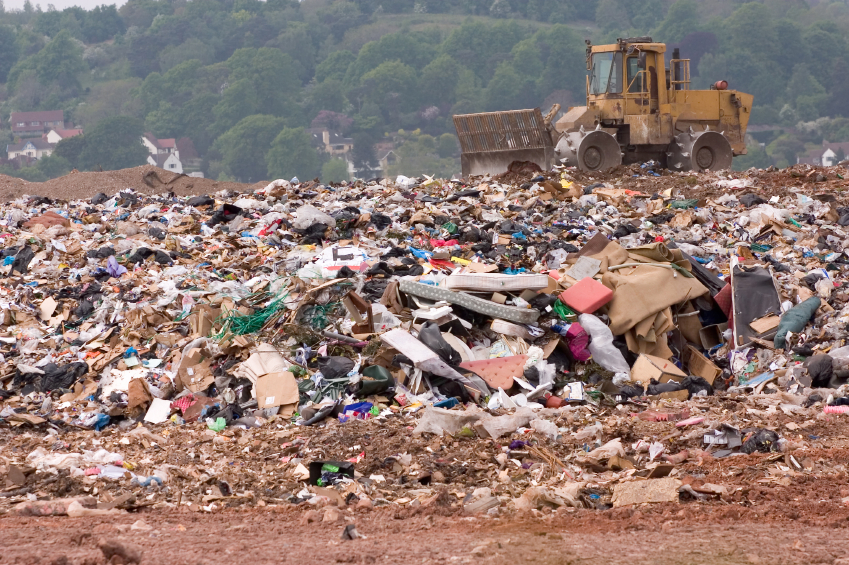
\includegraphics[scale=1]{Imagenes/Contaminacion_03.jpg}
\end{figure}
\end{frame}
\begin{frame}
\frametitle{Contaminación del Aire}
\vspace*{-1cm}
\begin{figure}
    \centering
    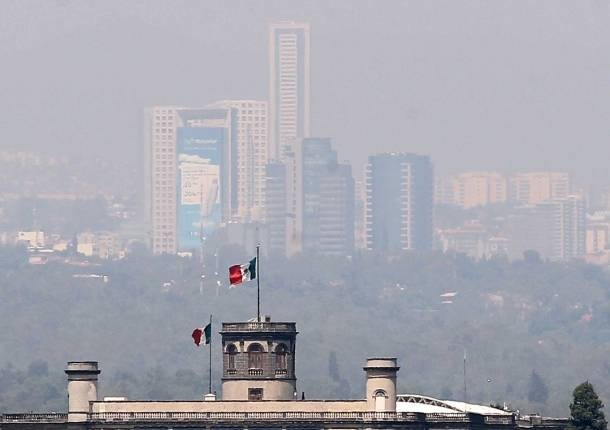
\includegraphics[scale=0.6]{Imagenes/Contaminacion_04.jpg}
\end{figure}
\end{frame}
\begin{frame}
\frametitle{Contaminación por Electrónicos}
\vspace*{-1cm}
\begin{figure}
    \centering
    
\includegraphics[scale=0.25]{Imagenes/Contaminacion_05.jpg}
\end{figure}
\end{frame}

\section{Consideraciones}
\frame{\tableofcontents[currentsection, hideothersubsections]}
\subsection{Trabajo en equipo}

\begin{frame}
\frametitle{Integrantes por equipo}
Cada poster se puede elaborar en equipo hasta de 3 integrantes.
\end{frame}
\begin{frame}
\frametitle{Presentación del poster}
Cada poster se montará en el Campus el día 22 de abril.
\end{frame}

\section{Evaluación}
\frame{\tableofcontents[currentsection, hideothersubsections]}
\subsection{Puntaje}

\begin{frame}
\frametitle{Puntos a otorgar}
El trabajo otorgará hasta \num{10} puntos de Evaluación Continua.
\end{frame}
\begin{frame}
\frametitle{Rúbrica}
Tendrán una rúbrica en donde se indicarán los elementos a incluir, así como el nivel de desempeño esperado.
\end{frame}
\begin{frame}
\frametitle{Entrega en físico}
El poster se entregará en físico en la clase del viernes 19 de abril.
\end{frame}

\end{document}